\documentclass[Main]{subfiles}

\begin{document}
\section*{Problem 1}

\paragraph{1. Determine the channel transition matrix (Hint: the channel has three
outputs.) and draw the channel model diagram.}

The diagram is as follow in Figure \ref{fig:1}.
\begin{figure}[H]
\centering
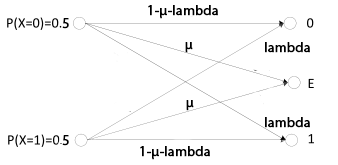
\includegraphics[scale=0.8]{part1}
\caption{Channel model diagram}
\label{fig:1}
\end{figure}

The input = 
\begin{ArgMat}
0.5 \\
0.5
\end{ArgMat}
\\
\\
The output =
\begin{ArgMat}
1-\lambda-\mu & \mu & \lambda\\
\lambda & \mu & 1-\lambda-\mu 
\end{ArgMat}

\paragraph{2. Determine the output entropy H(Y).}
The output entropy, $H(Y)$ is determined as follow:
\begin{align*}
H(Y) &= \sum_j P(y_j)\cdot log_2 \bigg[\dfrac{1}{P(y_j)}\bigg]\\
\text{where}\\
P(Y) &= \sum_{i=1}^u P_{i1} \cdot P(x_i)
\end{align*}

Given, that there's no real numbers as input, the symbolic values are calculated in \texttt{Matlab}.
\begin{align*}
P(Y=0) &= 0.5- \dfrac{\mu}{2}\\
P(Y=error) &= \mu\\
P(Y=1) &= 0.5- \dfrac{\mu}{2}\\
H(Y) &= \dfrac{\mu \cdot log\frac{1}{\mu}}{log(2)} - \dfrac{2\cdot log\bigg(\dfrac{-1}{\frac{\mu }{2}- 0.5} \bigg)\cdot \Big(\frac{\mu}{2}-0.5\Big)}{log(2)}
\end{align*}
If we had assigned some values to the output, as in part 4 
\begin{ArgMat}
0.7 & 0.2 & 0.1\\
0.1 & 0.2 & 0.7
\end{ArgMat}, the result of $H(Y)$ would be 1.5219


\paragraph{3. Determine the mutual information I(X, Y).}
To calculate the mutual information we use the following formula:
\begin{align*}
I(X,Y) &= H(Y) - H(Y/X)\\
\text{where}\\
H(Y/X) &= \sum_{i,j} P(x_i, y_j) \cdot log_2\bigg[\dfrac{1}{P(x_i/y_j)}\bigg]\\
\text{and}\\
P(x_i, y_j) &= P(x_i/y_j) \cdot P(y_j)\\
\text{and}\\
P(x_i/y_j) &= \dfrac{P(y_j/x_i)\cdot P(x_i)}{\sum_{i=1}^U P(y_j/x_i)\cdot P(x_i)}
\end{align*}
Without all the subcalculations:
\begin{align*}
H(Y/X) &= \dfrac{l\, \mathrm{log}\!\left(\frac{1}{\lambda}\right)}{\mathrm{log}\!\left(2\right)} - \dfrac{2\, \mathrm{log}\!\left(-\frac{1}{l + \mu - 1}\right)\, \left(\frac{\lambda}{2} + \frac{\mu}{2} - \frac{1}{2}\right)}{\mathrm{log}\!\left(2\right)} + \frac{\mu\, \mathrm{log}\!\left(\frac{1}{\mu}\right)}{\mathrm{log}\!\left(2\right)}
\\
I(X,Y) &= \dfrac{2\, \mathrm{log}\!\left(-\frac{1}{\lambda + \mu - 1}\right)\, \left(\frac{\lambda}{2} + \frac{\mu}{2} - \frac{1}{2}\right)}{\mathrm{log}\!\left(2\right)} - \dfrac{2\, \mathrm{log}\!\left(-\frac{1}{\frac{\mu}{2} - \frac{1}{2}}\right)\, \left(\frac{\mu}{2} - \frac{1}{2}\right)}{\mathrm{log}\!\left(2\right)} - \dfrac{\lambda\, \mathrm{log}\!\left(\frac{1}{\lambda}\right)}{\mathrm{log}\!\left(2\right)}
\end{align*}

However, if we use the the numbers from question 2 we get the following:
\begin{align*}
H(Y,X) &= 1.1568\\
I(X,Y) &=0.3651
\end{align*}

\paragraph{4. If $\lambda = 0.1$ and $\mu = 0.2$, what is the channel capacity?}

The channel capacity can be calculated as follow:
\begin{align*}
C_s &= I_{max}(X,Y) & \\
	&= H_{max}(Y) - H(Y/X)\\
	\text{where}\\
H_{max}(Y) &= \sum_{i=0}^2 P(y_i)log_2\bigg[\dfrac{1}{P(y_i)}\bigg]
\end{align*}
$H_{max}(Y)$ is calculated by letting the probability of $x_1$ and $x_2$ have the same value, which they do in this case.
\begin{align*}
H_{max}(Y) &= 1.5219\\
C_s &= 1.5219 - 1.1568 = 0.3651
\end{align*}






























\end{document}